%\documentclass[conf]{new-aiaa}
\documentclass[journal]{new-aiaa} %for journal papers
\usepackage[utf8]{inputenc} % Used by Colin
\usepackage{xcolor} % Used by Colin
\usepackage{soul} % Used by Colin

\usepackage{graphicx} % Used by Colin
\usepackage{amsmath} % Used by Colin
\usepackage[version=4]{mhchem} % Used by Colin
\usepackage{siunitx} % Used by Colin
\usepackage{longtable,tabularx} % Used by Colin
\setlength\LTleft{0pt} % Used by Colin

% Custom packages
\usepackage{subcaption} % Used by Colin
\usepackage{makecell}
\usepackage{comment}

% Packages to allow InkScape Text to Display and Autoformat in figures
\graphicspath{{Photos/}{Photos/MUFASA/}{Photos/Figures/}} % The subfolders where images are stored

\usepackage{multirow} % Allows for multirow table entries
\usepackage{array} % Allows for centered table entries
\usepackage{booktabs} % Allows for centered table entries
\usepackage{threeparttable} % Aligns table caption to be the width of the table
\usepackage{matlab-prettifier} % Allows for the addition of MATLAB code
\usepackage{glossaries}

\usepackage{pdfpages} % Allows for inclusion of other PDFs

\usepackage[nameinlink]{cleveref}
\crefformat{equation}{#2Eq.~#1#3} % adjust what the command \cref{label}
\crefformat{figure}{#2Fig.~#1#3} % adjust what the command \cref{label} displays for figures displays for figures

\title{Writing and \LaTeX\ Tips for academic writing in the AERO-CORE Lab} %Title to be <= 12 words as per: https://www.aiaa.org/publications/journals/Journal-Author#follow-the-minimum-formatting-requirements

\author{
	Benjamin Durante\footnote{MSc, Department of Mechanical and Manufacturing Engineering}
}
\affil{University of Calgary, Calgary, Alberta, Canada, T2N 4V8}

\begin{document}

\newcommand{\MufasaLength}{1.30}
\newcommand{\MufasaWidth}{0.96}
\newcommand{\MufasaWeight}{51.6}
\newcommand{\MAC}{c_{\textup{mean}}}
\newcommand{\MACone}{c_{\textup{mean}_{1}}}
\newcommand{\MACtwo}{c_{\textup{mean}_{2}}} % Document containing variables used throughout

	\maketitle
	\begin{center}
		Revision 2
		
		\today
	\end{center}
	% PURPOSE: Each full-length paper must have a summary-type abstract of 100 to 200 (maximum) words in one paragraph, without numerical references, acronyms, or abbreviations. The abstract indicates the subjects dealt with in the paper and states the objectives of the investigation.
% SOURCE: https://www.aiaa.org/publications/journals/Journal-Author#follow-the-minimum-formatting-requirements
\begin{abstract}
	Writing and \LaTeX\ tips are presented to guide future document creation. 
	Writing best practices are addressed, along with common writing errors to avoid. 
	A summation of useful \LaTeX\ functions is presented to reduce coding errors and increase writing efficiency. 
	Finally a holistic suggestion for the writing process is reviewed. 
	The first sentence in the abstract is the most important sentence in a document. 
	The first sentence is what people will read first, and is what they will use to determine if the paper is relevant or worth reading. 
	The first sentence should describe the overall purpose of the paper, or what was performed. 
	The rest of the abstract acts as a condensed paper, discussing the high-level process and results.  
\end{abstract}
	\tableofcontents
	\newpage
	\section{Nomenclature}

The nomenclature should be laid out according to the journal/conference/thesis requirements. 
Common nomenclatures sections include: Abbreviations, Symbols, Greek Symbols, Roman Symbols, Subscripts, and Superscripts. 
Within each of these nomenclature sections, symbols are organized alphabetically. 
An example nomenclature is presented in this section, however, always refer to the formatting requirements of where a document is being submitted to. \\

{\renewcommand\arraystretch{1.0}
\noindent 
Symbols
	\noindent\begin{longtable*}{@{}l @{\quad=\quad} l@{}}
		%$C_{D}, C_{L}, C_{Y}$ & drag, lift, and lateral force coefficient \\
		%$C_{F}$ & skin friction coefficient \\
		%$C_{l}, C_{m}, C_{n}$ & roll, pitch, and yaw moment coefficient \\
		$\MAC$ & mean aerodynamic chord, m \\
		$\textbf{F}_{\textup{aero}}$ & aerodynamic force vector along the body axes, N\\
		$\textbf{F}_{g}$ & force of gravity vector, N \\
		$\textbf{F}_{\textup{net}}$ & total force vector, N\\
		$\textbf{F}_{T}$ & force vector of engine thrust, N
\end{longtable*}
\noindent
Greek Symbols
\noindent\begin{longtable*}{@{}l @{\quad=\quad} l@{}}
	$\alpha$ & angle of attack, rad \\
	$\beta$ & angle of sideslip, rad \\
	%$\delta_{a}$ & aileron deflection angle \\
	%$\delta_{e}$ & elevator deflection angle \\
	%$\delta_{el}$ & left elevon deflection angle \\
	%$\delta_{er}$ & right elevon deflection angle \\
	%$\delta_{r}$ & rudder deflection angle \\
	%$\delta_{T}$ & throttle position setting between 0 and 1 \\
	$\delta_{a}, \delta_{e}, \delta_{r}$ & control surface deflections, rad
\end{longtable*}}
\noindent
Subscripts
{\renewcommand\arraystretch{1.0}
	\noindent\begin{longtable*}{@{}l @{\quad=\quad} l@{}}
		$0$ & nominal coefficient 
\end{longtable*}}
\noindent
\begin{comment}
Superscripts
{\renewcommand\arraystretch{1.0}
	\noindent\begin{longtable*}{@{}l @{\quad=\quad} l@{}}
		%$\bar{\pbox{1}}$ & variable vector \\
		%$\dot{\pbox{1}}$ & variable derivative with respect to time \\
		$\hat{\pbox{1}}$ & normalized variable
\end{longtable*}}
\end{comment}

\begin{comment}
\noindent \textit{Subscript/Superscript}
{\renewcommand\arraystretch{1.0}
\noindent\begin{longtable*}{@{}l @{\quad=\quad} l@{}}
$0$ & nominal coefficient \\
$P$ & coefficient as a function of vehicle roll-rate \\ 
$Q$ & coefficient as a function of vehicle pitch-rate \\ 
$R$ & coefficient as a function of vehicle yaw-rate \\
$\alpha$ & coefficient as a function of angle of attack \\
$\alpha^2$ & coefficient as a function of the square of angle of attack \\
$\beta$ & coefficient as a function of angle of sideslip  \\ 
$\delta_{a}$ & coefficient as a function of aileron deflection angle \\
$\delta_{e}$ & coefficient as a function of elevator deflection angle \\
$\delta_{e}^{2}$ & coefficient as a function of the square of elevator deflection angle \\
$\delta_{r}$ & coefficient as a function of rudder deflection angle \\
$\dot{}$ & variable derivative with respect to time
\end{longtable*}}
\end{comment}
	\section{Writing}

\lettrine{C}{lear} and concise writing is critical in science to convey research, making it a paramount skill to exercise. 
This section outlines advice, tips, and suggestions to consider when writing. 
The writing instruction provided is in no way conclusive, however, it is the author's hope that this document will be developed through time to ease students into the expectations of academic writing. 
Sources that go more in-depth on writing instruction include work by \citeauthor{natureWritingTips} \cite{natureWritingTips}, \citeauthor{writingSpringer} \cite{writingSpringer}, and \citeauthor{writingAIAA} \cite{writingAIAA}.

\subsection{Document Setup}

The most important thing to consider before even beginning to write is \textit{what are the expectations}. 
Every technical writing conference/journal/thesis will have a set of formatting requirements \cite{writingAIAA,writingThesisUofC}. 
Review these requirements \textbf{before} writing to save time re-formatting everything later. 
These organizational formatting requirements are the be-all-end-all to discussions about formatting, the document must align with the requirements. 

\subsubsection{Tense}

Tense is a common simple mistake that is easily correctable by considering the intent of the information. Tense is determined by what the sentence is describing \cite{natureWritingTips}, common sentence types and their associated tense are presented in \Cref{tab:tenseBasedOnSentence}. 

\begin{table}[hbt!]
	\centering
	\begin{threeparttable}[b]
		\caption{How tense changes based on the intent of the sentence \cite{natureWritingTips}. \label{tab:tenseBasedOnSentence}}
		\begin{tabular}{cc}
			\toprule
			\textbf{Sentence Describes} & \textbf{Tense} \\ \midrule
			Work done & \multirow{3}{*}{Past} \\
			Work reported &  \\
			Observations &  \\ \midrule
			General truths & \multirow{2}{*}{Present} \\
			Atemporal facts &  \\ \midrule
			Perspectives & Future \\ \bottomrule
		\end{tabular}
	\end{threeparttable}
\end{table}

\noindent
Loose tense guidance is also inferred from what section of a scientific report the sentence is in. 
General tense guidance based on typical scientific writing sections is presented in \Cref{tab:tenseBasedOnSection}. 
Exceptions to \Cref{tab:tenseBasedOnSection} do exist, and as such this table should only be used as a guide. 
One such major exception is that the present tense is always used when a specific result, figure, table, or paper is the subject of a sentence (as demonstrated throughout this document). 

\begin{table}[hbt!]
	\centering
	\begin{threeparttable}[b]
		\caption{General tense usage in scientific writing sections \cite{tenseScientificWriting}. \label{tab:tenseBasedOnSection}}
		\begin{tabular}{cc}
			\toprule
			\textbf{Section} & \textbf{Tense} \\ \midrule
			Abstract & Past \\
			Introduction & Present \\
			Literature Review & Past and Present \\
			Methods & Past \\
			Results & Past \\
			Discussion & Past, Present, and Future \\
			Conclusion & Past, Present, and Future \\ \bottomrule
		\end{tabular}
	\end{threeparttable}
\end{table}


\subsubsection{Figures and Tables} \label{sec:documentSetupFigureTableRules}

Figures and tables are useful tools to present complex visual data, or relate two concepts graphically. 
General presentation norms and rules exist that apply to figures and tables. 
A couple of these shared norms are listed here: 
\begin{itemize}
	\item Figures and tables must always be introduced in-text before they are presented, 
	\item Figures and tables should not have titles, 
	\item Figure and table text should match document size and font, 
	\item Captions should remain within the margins of the figure/table they describe, 
	\item Captions should be sufficiently descriptive to know what the figure will contain without viewing it, 
	\item Captions should end with a period (as they are a proper sentence).
\end{itemize}

\noindent
Specific figure considerations include: 
\begin{itemize}
	\item Colour should be chosen in such a way that data will still be differentiable in greyscale,
	\item Gradient colour should start/end light/dark, not have white in the middle of the gradient as this could become confusing in greyscale, an example of gradients is presented in \cref{fig:gradientExample},
	\item Ideally, different data symbols should be utilized to ensure data is differentiable in greyscale, 
	\item Colour choice should be considerate of colourblind people \cite{colourScienceMisuse},
	\item Sub-figures require captions, 
	\item Axes labels should be present and contain units, 
	\item Axes should end on definitive numbers. 
\end{itemize}

\noindent
Examples of these aforementioned norms are presented in \cref{fig:gradientExample} and \ref{fig:dataExample}. 
How to create figures is discussed in \Cref{sec:figureCreation}. 

The significance of a figure/table should always be discussed just prior, or just after it is introduced. 
As per A. Ramirez-Serrano (personal communication, March 22, 2022), it is the author's responsibility to ``digest'' the figure information and clearly present the important elements to the reader. 


\begin{figure}[hbt!]
	\centering
	\captionsetup{width=\textwidth}
	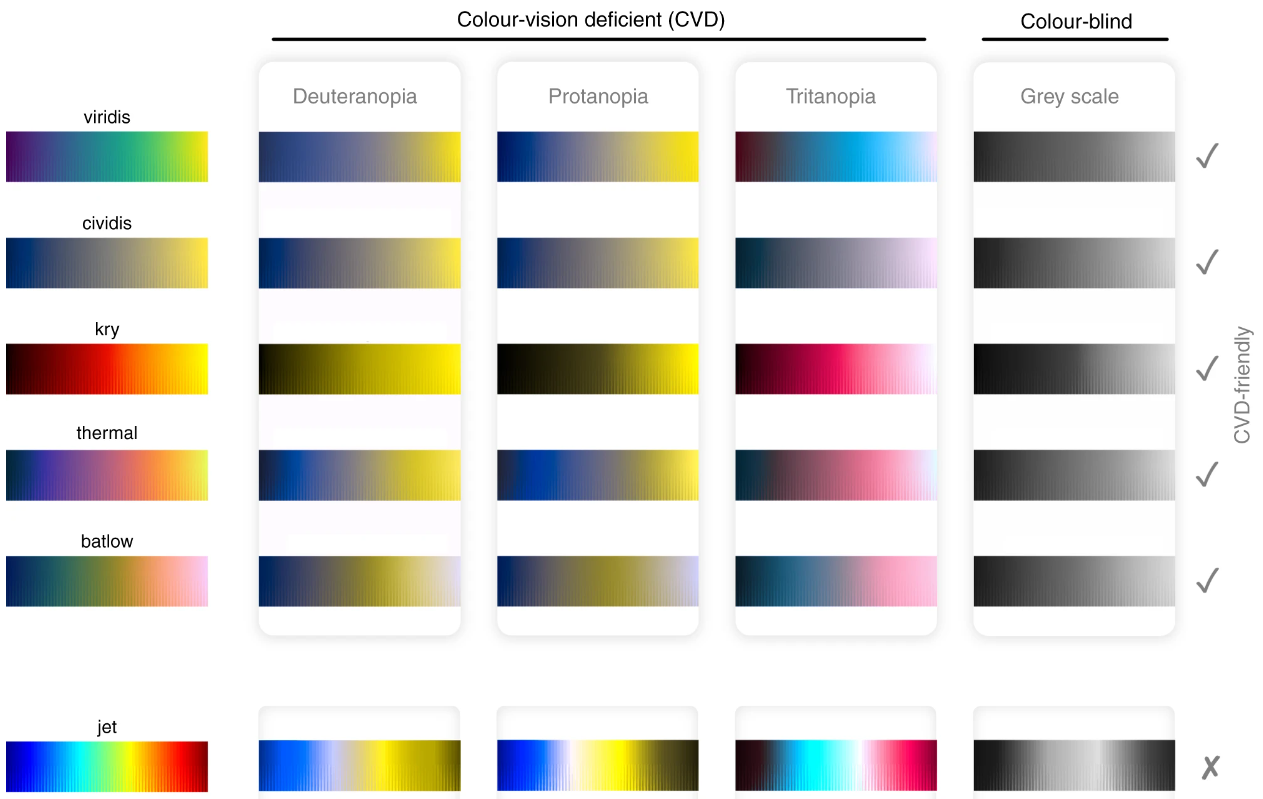
\includegraphics[width=\textwidth]{Photos/Figures/gradients.png}
	\caption{How common gradients appear to various colourblind diagnoses, adapted from \citeauthor{colourScienceMisuse} \cite{colourScienceMisuse}.}
	\label{fig:gradientExample}
	\hfill
\end{figure}



\begin{figure}[hbt!]
	\centering
	\captionsetup{width=0.5\textwidth}
	\def\svgwidth{0.55\textwidth}
	\input{Photos/Figures/MUFASAandGoJettandTranceRelationshipComparison-InverseTimeConstant-MachNumber-2column_Editted.eps_tex}
	\caption{MUFASA B aerodynamic design and coordinate system \cite{BenThesis}. Notice how different symbols and colours are used. Also note how the ends of the x and y axes are denoted by a number and not left ambiguously floating.}
	\label{fig:dataExample}
	\hfill
\end{figure}

\subsubsection{Equations}

Equations are similar to figures and tables in that they are addressed in-text prior to their presentation. 
Unless otherwise stated, the first time a variable is used in an equation it is presented in-text before or just after the equation. 
Exceptions to the rule do exist inline with formatting guidelines specific to the conference/journal/thesis being written. 
An example equation highlighting how aerodynamic forces are added is presented in \cref{eqn:netForce}, 

\begin{equation} \label{eqn:netForce}
	F_{\text{net}} = F_{\text{aero}} + F_{\text{g}} + F_{\text{T}}
\end{equation}

\noindent where $F_{\text{net}}$, $F_{\text{aero}}$, $F_{\text{g}}$, and $F_{\text{T}}$ represent net force, aerodynamic force, gravitational force, and thrust force, respectively. 

\subsection{General Writing}

Common writing mistakes and misconceptions are presented in this section. It is the authors hope this list is useful (and error-free). 
Great writing resources are found online \cite{writingAIAA}, and at the University of Calgary \cite{writingUofC,writingCoursesUofC}. 
The \citeauthor{writingUofC} \cite{writingUofC} in particular is a great resource for 1-on-1 writing help and support, with extremely knowledgeable staff. 
It is strongly recommended to seek assistance \textbf{BEFORE} completing a document. By requesting feedback early, more time can be spent writing properly instead of editing what has already been written. 

\subsubsection{Sentence Structure}
Conciseness is key in academic writing, readers ``want to find the relevant information quickly and efficiently,'' \cite{writingSpringer}. 
Sentences should only contain \textbf{one idea}, and be no longer than 20-25 words in length \cite{writingSpringer}. 


\subsubsection{Language}

A conference/journal/thesis requires exact language be used. 
Using words such as \textit{can}, \textit{could}, and \textit{would} make the document sound uncertain. 
This type of uncertain wording should only be used when discussing future work, which is always inherently uncertain. 
Do not write "\textit{...this can be seen in Fig...,}", instead write "\textit{...this is presented in Fig...}".

A word on the use of the word \textit{this}. 
The word \textit{this} should not start a sentence unless it is followed directly with an indication of what \textit{this} is. 
A sentence should be a standalone idea, thus, without reiterating to the reader what \textit{this} is, it is very easy for the reader to become confused. 
Parallel to this concept of the uncertainty of \textit{this} is how authors sometimes use \textit{it} without explaining what \textit{it} is they are referring to. 

Word choice is paramount and matters. While often used interchangeably in normal language, \textit{compute}, \textit{evaluate}, and \textit{calculate} suggest very different approaches were taken. Consider what verbs are being used throughout the document and what they imply. 


\subsubsection{Commas}

Always use the Oxford comma when making a list. The Oxford comma helps the reader understand if the last two items in a list are together or separate. 

Commas should also be used after transition words, such as ``..., however,...''. 


\subsection{Referencing}

Referencing is a vital part of science, a way to track that all scientific statements are supported by evidence \cite{referncingVirtues}. 
It is imperative that references are used properly and correctly associated to the factual information they are related to. 
As stated by \citeauthor{referncingVirtues} \cite{referncingVirtues}:
\begin{quotation}
	\noindent
	A reference citation is supposed to provide accurate underpinning for a statement and to represent the current state of research, or, in the case of a maverick opinion, to ensure it is recognizable as such. \cite{referncingVirtues}
\end{quotation} 

\noindent
Some good rules of thumb to guide if you need to reference a statement are: 
\begin{itemize}
	\item Did you perform the task/experiment?
	\item If commenting about an industry trend, do you have years of first-hand experience in that industry?
	\item Is the statement common knowledge (ie. it is a first year taught engineering concept/fact)?
	\item Did you develop this equation, figure, diagram? 
	\item Was the idea, method, statement learnt from another source (ie. a textbook or article)?
\end{itemize}
\noindent
If the answer to any of the first four is no, or the last is yes, then you \textbf{NEED} a reference. 
If a reference cannot be found to support a statement, either the statement is incorrect, or it is too broad and should be reworded to be more defensible. 

References are placed at the end of a sentence if describing a single idea, if describing multiple ideas, referencing is placed just behind the idea it is associated with. 
Proper referencing is also a topic formally covered by the \citeauthor{writingUofC} \cite{writingUofC} and \citeauthor{writingCoursesUofC} \cite{writingCoursesUofC}.
	\section{\LaTeX~Coding Best Practices} \label{sec:Conclusion}
This section outlines some key coding functions that are extremely helpful when working with \href{https://www.latex-project.org/}{\LaTeX}. 
For readers new to \LaTeX\, ``LaTeX\ is a high-quality typesetting system; it includes features designed for the production of technical and scientific documentation,'' \cite{latexExplanation}. 
\LaTeX\ is written via the use of an editing software. 
Common editing programs include \href{https://www.overleaf.com/}{OverLeaf} for online usage, or \href{https://miktex.org/}{Mik\TeX} with \href{https://www.texstudio.org/}{\TeX studio} for offline usage. 

\subsection{Document Setup}
Long \LaTeX\ documents become very confusing, very quickly if a proper file structure is not established. 
\LaTeX\ uses one document to import required packages, set formats, and generate a .PDF document. 
It is suggested to use the main \LaTeX\ document only for the global packages, and the calling of subsequent document files. 
Therefore, limited writing should occur within the main \LaTeX\ file. 
Sections of a document should be individual files, added to the main file via the command \verb*|\input{}|. 
An example file structure, with \LaTeX\ files in the main folder, and supporting photos and resources in sub-folders, is presented in \cref{fig:documentSetupExample}.


\begin{figure}[hbt!]
	\centering
	\captionsetup{width=0.6\textwidth}
	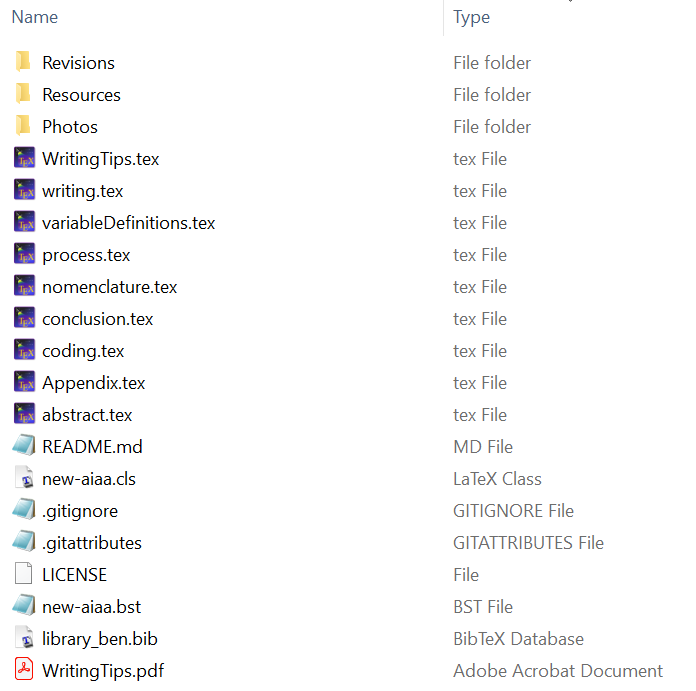
\includegraphics[width=0.6\textwidth]{Photos/Figures/projectStructure.png}
	\caption{Example file structure for a \LaTeX\ document project.}
	\label{fig:documentSetupExample}
	\hfill
\end{figure}

\noindent
In \cref{fig:documentSetupExample}, the main \LaTeX\ file is named \textit{WritingTips.tex}. 
This main file then imports code written in the remaining .TEX files. 
File types ending with .CLS and .BST are files used to automatically format the main document. 
File types ending with .BIB is for the \href{https://www.bibtex.org/}{Bib\TeX} bibliography entries. 

\subsection{Useful Command Packages}

A list of useful \LaTeX\ command packages not always included in \LaTeX\ templates are detailed in \Cref{tab:usefulPackagesText,tab:usefulPackagesFiguresTables,tab:usefulPackagesMath}. 
The packages presented in \Cref{tab:usefulPackagesText,tab:usefulPackagesFiguresTables,tab:usefulPackagesMath} are in no-way representative of all packages in existence, however, they have been included here due to the usefulness they have previously provided the author. 

\begin{table}[hbt!]
	\centering
	\begin{threeparttable}[b]
		\caption{Useful \LaTeX\ packages related to document text.}
		\label{tab:usefulPackagesText}
		\begin{tabular}{ll}
			\toprule
			\textbf{Package} & \textbf{Description} \\ \midrule
			\href{https://ctan.org/pkg/natbib}{natbib} & Bibliography style formatting \\
			\href{https://ctan.org/pkg/glossaries}{glossaries} & Glossary/nomenclature/symbol referencing \\
			\href{https://ctan.org/pkg/hyperref}{hyperref} & For linking references within the text \\
			\href{https://ctan.org/pkg/cleveref}{cleveref} & Smarter in-text referencing \\ 
			\href{https://ctan.org/pkg/comment}{comment} & Comment out sections of \LaTeX\ code \\
			\href{https://ctan.org/pkg/rotating}{rotating} & For rotating text/figures/tables \\
			\href{https://ctan.org/pkg/draftwatermark}{draftwatermark} & Creates a watermark over every page \\
			\bottomrule
		\end{tabular}
	\end{threeparttable}
\end{table}

\begin{table}[hbt!]
	\centering
	\begin{threeparttable}[b]
		\caption{Useful \LaTeX\ packages related to document figures and tables.}
		\label{tab:usefulPackagesFiguresTables}
		\begin{tabular}{ll}
			\toprule
			\textbf{Package} & \textbf{Description} \\ \midrule
			\href{https://ctan.org/pkg/graphicx}{graphicx} & For figures \\
			\href{https://ctan.org/pkg/float}{float} & For figure placement \\
			\href{https://ctan.org/pkg/caption}{caption} & Allows for sub-figures \\
			\href{https://ctan.org/pkg/subcaption}{subcaption} & Allows for sub-figures \\
			\href{https://ctan.org/pkg/color}{color} & Package required for InkScape text \\
			\href{https://ctan.org/pkg/threeparttable}{threeparttable} & Aligns table caption to be the width of the table \\
			\href{https://ctan.org/pkg/booktabs}{booktabs} & Allows for centered table entries \\
			\href{https://ctan.org/pkg/array}{array} & Allows for centered table entries \\
			\href{https://ctan.org/pkg/multirow}{multirow} & Allows for multirow table entries \\
			\bottomrule
		\end{tabular}
	\end{threeparttable}
\end{table}


\begin{table}[hbt!]
	\centering
	\begin{threeparttable}[b]
		\caption{Useful \LaTeX\ packages related to document math.}
		\label{tab:usefulPackagesMath}
		\begin{tabular}{ll}
			\toprule
			\textbf{Package} & \textbf{Description} \\ 
			\midrule
			\href{https://ctan.org/pkg/amsmath}{amsmath} & For extra math utilities \\
			\href{https://ctan.org/pkg/amssymb}{amssymb} & For math symbols and fonts \\
			\href{https://ctan.org/pkg/cancel}{cancel} & For crossing out terms in equations \\
			\href{https://ctan.org/pkg/bm}{bm} & For bold mathematical symbols \\
			\href{https://ctan.org/pkg/siunitx}{siunitx} & For SI units in equations \\
			\href{https://ctan.org/pkg/empheq}{empheq} & To box multi-line equations \\ 
			\bottomrule
		\end{tabular}
	\end{threeparttable}
\end{table}


\subsection{Nomenclature} \label{sec:nomenclatureLaTeXCode}

\newacronym{SSUAV}{SSUAV}{Small-scale Supersonic Uncrewed Aerial Vehicle}
\newglossaryentry{beta}{name={$\beta$},description={angle of sideslip}}
Nomenclature tracking is facilitated via the \textit{glossaries} package. 
The glossaries package allows for internal referencing of variables. 
The style of the nomenclature presented is controlled via the command \verb*|\newglossarystyle{name}{code}|. 
Acronyms and symbols are defined using the following two commands, respectively: 

\noindent
\verb*|\newacronym{label}{short}{long}| 

\noindent
\verb*|\newglossaryentry{label}{name={name},description={description}}|. 

\noindent
Variables are called in-text via the command \verb*|\gls{label}|. 
The first time a acronym is written using the \verb*|\gls{}| command it is fully spelled out, all subsequent references print only the acronym.  

\subsection{Internal Document Referencing}

\LaTeX\ automatically handles referencing using its built-in \verb*|\ref{}| or the often preferred \textit{cleveref} package \verb*|\cref{}|. 
How referencing works is a \verb*|\label{}| is placed at a section title (\verb*|\label{sec:}|), in an equation (\verb*|\label{eqn:}|), in a table (\verb*|\label{tab:}|), or in a figure (\verb*|\label{fig:}|). 
With a label in place, say in \cref{fig:mufasaB2}, the Cleveref is used to add a reference in text. For example, \cref{fig:mufasaB2} is labelled \textit{fig:mufasaB2}, so to reference \cref{fig:mufasaB2} in-text the code required is~\verb*|\cref{fig:mufasaB2}|.

\subsection{Citations} \label{sec:citations}

Always check the style and expected format of references for the journal/conference/university the paper will be submitted to. 
When citing, ensure the Bib\TeX\ file has all the required information to be displayed according to the journal/conference/university requirements. 
Unfortunately, the Bib\TeX\ data fields required vary slightly between referencing formats. It is suggested to be extra cognizant  of how the references are appearing when switching between referencing styles.  
An example Bib\TeX\ entry for work by \citeauthor{BenThesis} \cite{BenThesis} is provided in \Cref{sec:appendixBibTex}. 
Additional Bib\TeX\ entry formats are found online, with common types being \verb*|@article{}|, \verb*|@inproceedings{}|, \verb*|@techreport{}|, \verb*|@mastersthesis{}|, \verb*|@phdthesis{}|, \verb*|@book{}|, and \verb*|@misc{}|. 
 
Based on the Bib\TeX\ identification name (ex. \textit{BenThesis} in \Cref{sec:appendixBibTex}) references are easily cited in-text and added to the bibliography. 
Multiple commands are used to automatically cite a work depending on the presentation desired. 
Common \LaTeX\ commands, and their resulting text, are presented in \Cref{tab:citationCoding}.

\begin{table}[hbt!]
	\centering
	\begin{threeparttable}[b]
		\caption{\LaTeX\ commands and their resulting text using common citation formats. \label{tab:citationCoding}}
		\begin{tabular}{llll}
			\toprule
			\multicolumn{1}{c}{\multirow{2}{*}{\textbf{\LaTeX\ Command}}} & \multicolumn{3}{c}{\textbf{Citation Format}} \\
			\multicolumn{1}{c}{} & \multicolumn{1}{c}{\textbf{AIAA}} & \multicolumn{1}{c}{\textbf{IEEE}} & \multicolumn{1}{c}{\textbf{\begin{tabular}[c]{@{}c@{}}APA\\ (\textit{apalike})\end{tabular}}} \\ \midrule
			\verb*|\cite{BenThesis}| & \cite{BenThesis} & \cite{BenThesis} & Durante (2023) \\
			\verb*|\citep{BenThesis}| & \citep{BenThesis} & N/A & (Durante, 2023) \\
			\verb*|\citeauthor{BenThesis}| & \citeauthor{BenThesis} & \citeauthor{BenThesis} & \citeauthor{BenThesis} \\ \bottomrule
		\end{tabular}
	\end{threeparttable}
\end{table}


\subsection{Figure Creation} \label{sec:figureCreation}

Figures and diagrams should appear crisp, ideally they are vector files meaning they can be infinitely zoomed in without getting blurry. 
Examples of vector files include .PDF, .EPS, and .SVG. 
Diagram text should align with the document text exactly, as presented in \cref{fig:mufasaB2}. One way to ensure diagram text always matches the \LaTeX\ document text is by creating the diagrams in \href{https://inkscape.org/}{InkScape}. 
The diagram creation video is outlined in the following YouTube video: \url{https://youtu.be/NbHKJNMsYqE?si=W-XXTR8T_Izss_j1}. 
Note, this YouTube example only works for \href{https://inkscape.org/release/inkscape-1.1/?latest=1%29}{InkScape Version~1.1}. 
Figure \ref{fig:mufasaB2} is generated using the source code presented in \Cref{sec:appendixFigureSourceCode}. 

If it is not possible to use a vector file, a photo file such as .PNG is best. 
Attempt to avoid the use of .JPG files as the image displayed is more compressed and prone to blur. 


\begin{figure}[hbt!]
	\centering
	\captionsetup{width=0.7\textwidth}
	%\includegraphics[width=0.7\textwidth]{Photos/MUFASA/MUFASA-ISO-Frames-BodyLength.png}
	\def\svgwidth{0.7\textwidth}
	\input{Photos/MUFASA/MUFASA-ISO-Frames-BodyLength.eps_tex}
	\caption{MUFASA B aerodynamic design and coordinate system.}
	\label{fig:mufasaB2}
	\hfill
\end{figure}



If multiple related figures are presented than the \LaTeX\ \textit{subfigure} command should be used. 
An example of a subfigure is presented in \cref{fig:aircraftComparison}, with the associated source-code presented in \Cref{sec:appendixSubFigureSourceCode}. 

\begin{figure}[hbt!]
	\centering
	\begin{subfigure}{0.48\textwidth}
		\centering
		\captionsetup{width=0.95\linewidth}
		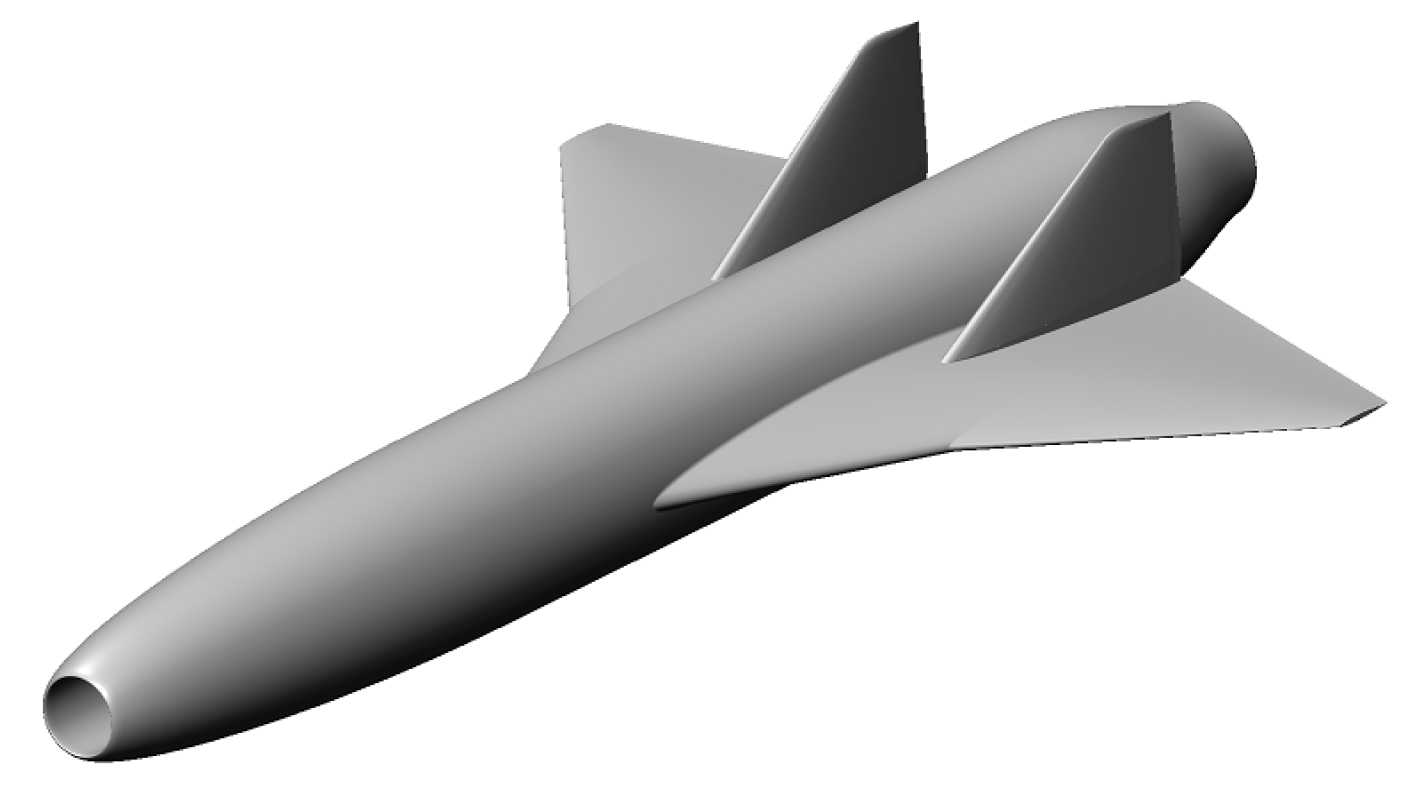
\includegraphics[width=0.95\linewidth]{Photos/Aircraft/MUFASA_Gair}
		\caption{MUFASA A.3, adapted from \citeauthor{ShaunThesis} \cite{ShaunThesis}.}
	\end{subfigure}
	\begin{subfigure}{0.48\textwidth}
		\centering
		\captionsetup{width=0.95\linewidth}
		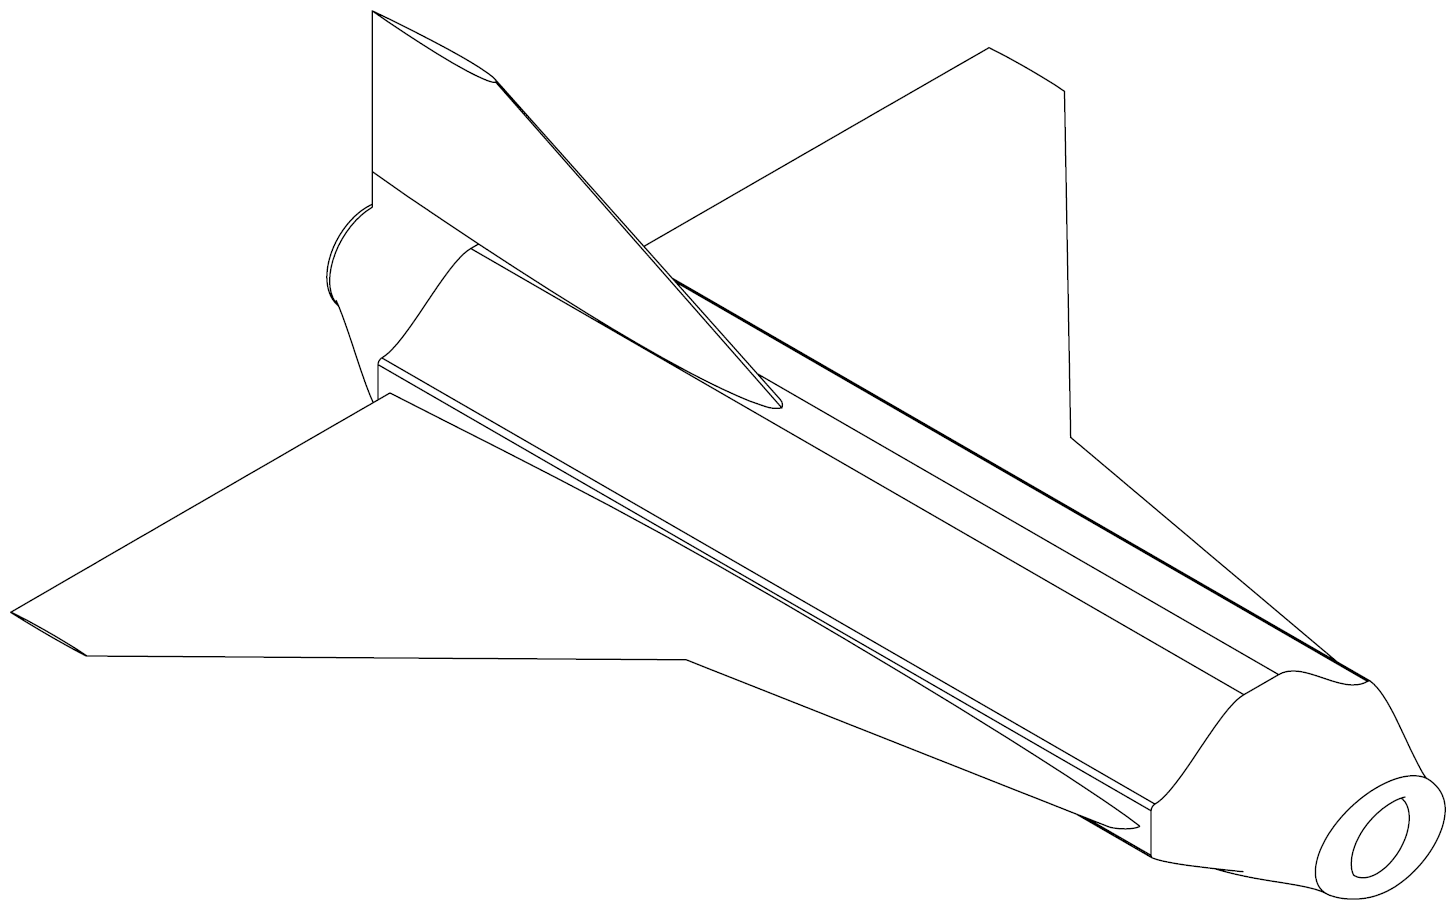
\includegraphics[width=0.95\linewidth]{Photos/Aircraft/MUFASA_ISO}
		\caption{MUFASA B.1.}
	\end{subfigure}
	\caption{MUFASA project aircraft versions (not to scale). \label{fig:aircraftComparison}}
\end{figure}

Matching the formatting of plotted results to the \LaTeX\ document they will be presented in is critically important. 
All rules provided in \Cref{sec:documentSetupFigureTableRules}, and exemplified in \cref{fig:dataExample} should be followed. 
An example of MATLAB code used to auto-format plotted data for \LaTeX\ is presented in \Cref{sec:appendixMatlabFigureCode}. 
It is also worth noting that plotted data could be directly drawn in \LaTeX\, using \LaTeX\ code, however this workflow requires first generating the plotted data in \href{https://www.python.org/}{Python} according to A. Garcia (personal communication, December 05, 2023).

\subsection{Table Creation}
Useful \LaTeX\ commands to generate tables meeting the requirements outlined in \Cref{sec:documentSetupFigureTableRules} are presented in this section. 
A useful package to generate tables with correct caption widths is \textit{threeparttable}. 
To generate correct thickness horizontal lines, the commands \verb*|\toprule|, \verb*|\midrule|, and \verb*|\bottomrule| are used. 
Manually typing table formatting is complex, and it is instead recommended to use a formatting tool, such as the \href{https://www.tablesgenerator.com/}{TablesGenerator website}. 
As an example, the code used to generate \Cref{tab:tenseBasedOnSection} is presented in \Cref{sec:appendixTables}. 


\subsection{Equations}
When coding an equation, carefully consider what is a variable and what is a label. 
Variables should be in math text, while labels should be in regular text. 
For example, in \cref{eqn:netForce}, $F_{\text{net}}$ is net force, not force as a function of variables $n \times e \times t$. 
Regular text can be inserted into an equation via the \verb*|\text{}| command. 


Sometimes equations are exceptionally long, or a matrix is too tall. Some commands that aid with unwieldy equations include \textit{smallmatrix}, \textit{sideways}, \textit{align}, and \textit{split}.	
An example of how to split a long equation is presented in \Cref{sec:appendixLongEquation}.


\LaTeX\ allows for the creation of multiple unique mathematical symbols. A comprehensive overview of possible \LaTeX\ symbols, and their associated commands, is presented in \Cref{sec:appendixLaTeXSymbols}. 

\subsection{Custom Variable Creation}
\newcommand{\ap}{ArduPilot}
Local \LaTeX\ document variables are a way to aid in typing repetitive words or numerical values. 
These custom variables also aid in document consistency when referring to repeated words or values. 
An example of using locally defined document variables is creating a command to represent the word \textit{ArduPilot}. 
Due to the letters in \textit{ArduPilot}, it is an awkward word to type and a coding shorthand is created using the command: \verb*|\newcommand{\ap}{ArduPilot}|. 
Now, by typing \verb*|\ap\|, the word \ap\ is seamlessly inserted into the text. 
Note that the \verb*|\| following the \verb*|\ap| indicates a space should be left following the word \ap.

\LaTeX\ variables also work when inserted into InkScape generated figures, as outlined in the following YouTube video: \url{https://youtu.be/r0G44lxhTwc?si=SVSKCUj6mTy4rGCN}. 
Using variables in a diagram increases writing efficiency as it reduces the need to manually regenerate diagrams to change a variable when using the workflow presented in \Cref{sec:figureCreation}. 


	\section{Process}

\subsection{Backups}
Backing-up a document should be a priority, not an afterthought. 
Rewriting a paragraph is unfortunate, rewriting an entire thesis would be soul crushing. 
Multiple backup methods exist such as \href{https://onedrive.live.com/login/}{OneDrive}, \href{https://www.dropbox.com}{DropBox}, \href{https://github.com/}{GitHub}, \href{https://www.overleaf.com/}{OverLeaf}, or physical local backups, to name a few. 
While one is good, it is suggested to use multiple backup methods should a device or service become unexpectedly unavailable. 
This backup method also applies to data, always ensure data is backed-up. 

\subsection{Revision Control}
Revision control refers to the process of tracking changes to a document, or structured information. 
When writing, revision control takes two forms, iterative and milestone revision control. 

Iterative revision control refers to tracking the small changes a document naturally undergoes. 
Maybe a paragraph was removed in error, instead of rewriting, proper revision control should allow the document to be rolled back to a state where that paragraph exists.
A very powerful program for this type of revision control is \href{https://github.com/}{GitHub}, which integrates with both physical machines and \href{https://www.overleaf.com/}{OverLeaf}.

Milestone revision control refers to when a document is in a state to be reviewed. 
As indicated by C. Johansen (personal communication, May 25, 2023), revisions should be denoted sequentially following R1, R2, R3. Documents with feedback will have the reviewer's initials appended to the filename. An example document filename on revision three that was reviewed by C. Johansen would appear as: \verb*|AIAA_Scitech2024_Abstract_RocketTests_Smith_R3_CJ.pdf|.
	\section{Conclusion}
Clear and concise writing is a skill that requires it be a forethought, not an afterthought. 
Understanding the writing process reduces frustrations and increases writing efficiency. 
Document expectations should be considered prior to beginning, feedback should be sought early on, and writing best practices should be implemented throughout. 
\LaTeX\ is a powerful tool to aid in final formatting, with multiple userpackages that exist. 
By combining all the topics presented in this document, it is the author's hope that the reader's documents will be more enjoyable to write, and easier to review. 

	

	%An Appendix, if needed, should appear before the acknowledgments.

	\section*{Acknowledgments}
	Funding for this work was provided by the AERO-CORE research group. 

	\bibliography{library_ben}
	
	\section{Appendix}

\subsection{Bib\TeX\ Format} \label{sec:appendixBibTex}
An example Bib\TeX\ entry for work by \citeauthor{BenThesis} \cite{BenThesis}. 
Note, this Bib\TeX\ reference has been formatted with data entries for the AIAA reference format.  

\begin{verbatim}
	@mastersthesis{BenThesis,
		author = {Durante, Benjamin Joseph},
		pages = {1--128},
		school = {University of Calgary]},
		title = {Flying and Handling Qualities of Small-Scale Supersonic Uncrewed Aerial Vehicles},
		note = {{Avaliable: \url{https://dx.doi.org/10.11575/PRISM/40789}}},
		type = {{[Master's} Thesis},
		year = {2023}
	}
\end{verbatim}

\subsection{Figures in \LaTeX} \label{sec:appendixFigureSourceCode}

Figure \ref{fig:mufasaB2} is generated using the following source code:

\begin{verbatim}
	\begin{figure}[hbt!]
		\centering
		\captionsetup{width=0.7\textwidth}
		%\includegraphics[width=0.7\textwidth]{Photos/MUFASA/MUFASA-ISO-Frames-BodyLength.png}
		\def\svgwidth{0.7\textwidth}
		\input{Photos/MUFASA/MUFASA-ISO-Frames-BodyLength.eps_tex}
		\caption{MUFASA B aerodynamic design and coordinate system.}
		%\caption[Short caption for list of figures]{This is the full caption that will appear 
			under the figure.}
		\label{fig:mufasaB2}
		\hfill
	\end{figure}
\end{verbatim}

\subsection{Sub-Figures in \LaTeX} \label{sec:appendixSubFigureSourceCode}

Figure \ref{fig:aircraftComparison} is generated using the following source code:

\begin{verbatim}
	\begin{figure}[hbt!]
		\centering
		\begin{subfigure}{0.48\textwidth}
			\centering
			\captionsetup{width=0.95\linewidth}
			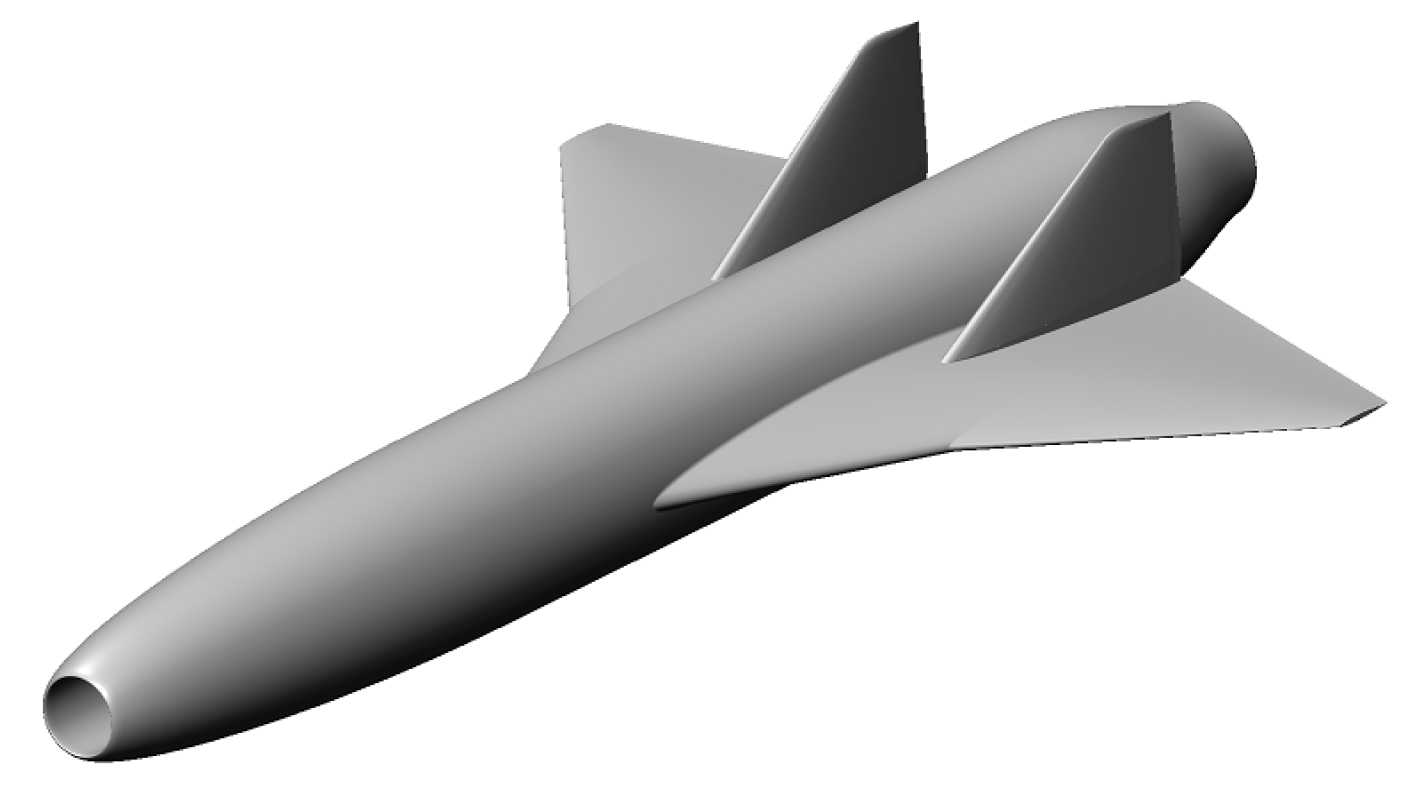
\includegraphics[width=0.95\linewidth]{Photos/Aircraft/MUFASA_Gair}
			\caption{MUFASA A.3, adapted from \citeauthor{ShaunThesis} \cite{ShaunThesis}.}
		\end{subfigure}
		\begin{subfigure}{0.48\textwidth}
			\centering
			\captionsetup{width=0.95\linewidth}
			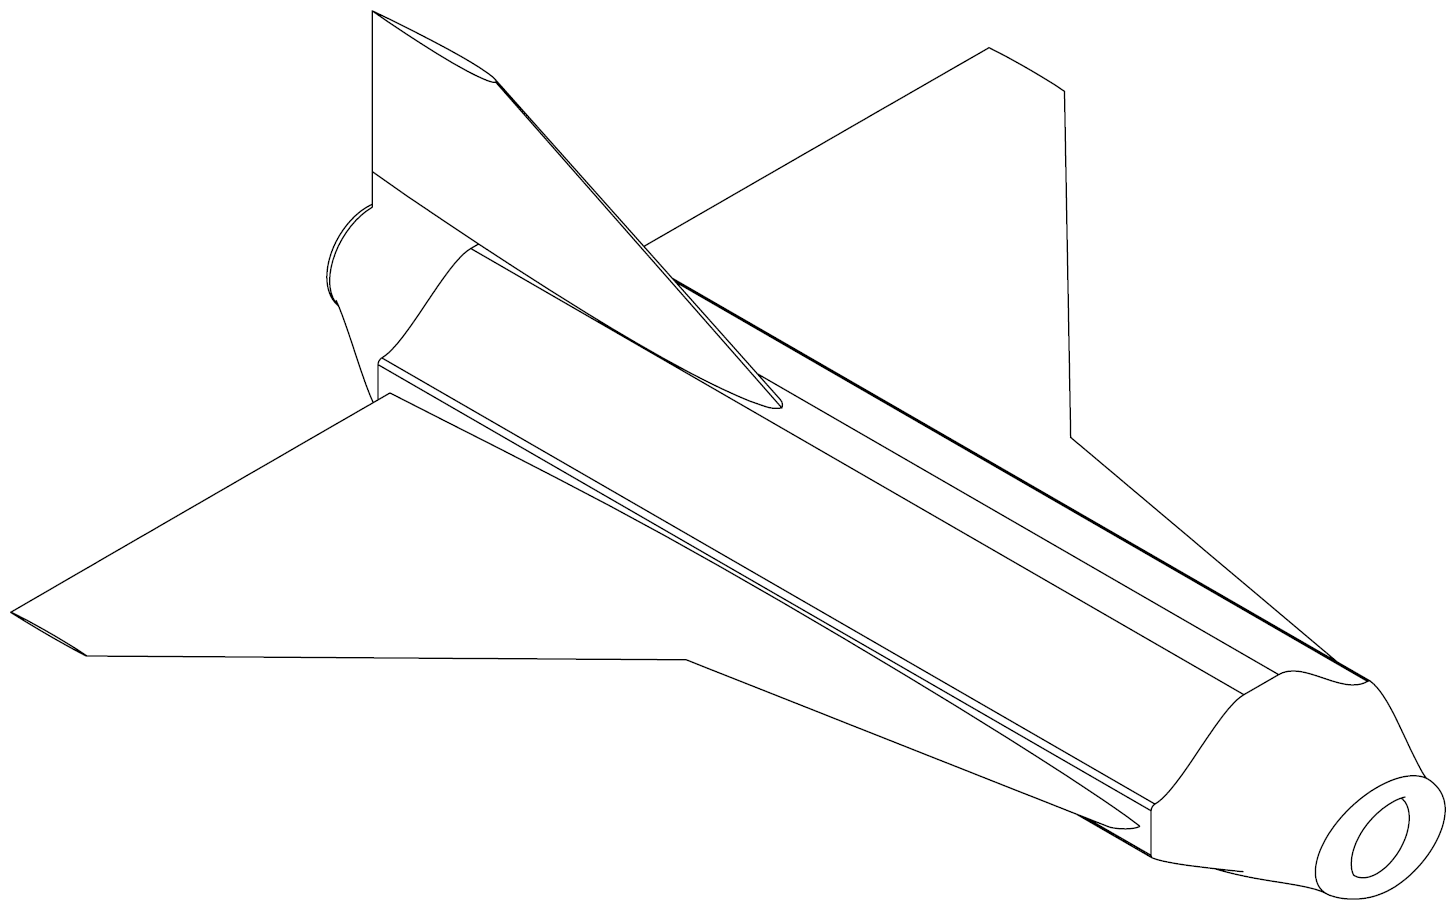
\includegraphics[width=0.95\linewidth]{Photos/Aircraft/MUFASA_ISO}
			\caption{MUFASA B.1.}
		\end{subfigure}
		\caption{MUFASA project aircraft versions (not to scale). \label{fig:aircraftComparison}}
	\end{figure}
\end{verbatim}

\subsection{MATLAB Figure Saving} \label{sec:appendixMatlabFigureCode}

The following MATLAB code automatically saves generated figures. 
The code adjusts the figure text and size, and saves each figure into three file types (.png, .eps, and .svg). 
The code requires that each figure generated has a unique figure name. The figure name from MATLAB is used as the filename, and is extremely useful once multiple result figures are displayed in one document. \cite{LaTeXSymbols}

\lstinputlisting[
frame=single,
numbers=left,
style=Matlab-editor
]{Photos/Code/SaveGeneratedFigures.m}

\subsection{Tables in \LaTeX} \label{sec:appendixTables}

\Cref{tab:tenseBasedOnSection} is generated using the following source code:

\begin{verbatim}
	\begin{table}[hbt!]
		\centering
		\begin{threeparttable}[b]
			\caption{General tense usage in scientific writing sections \cite{tenseScientificWriting}.}
			\label{tab:tenseBasedOnSection}
			\begin{tabular}{cc}
				\toprule
				\textbf{Section} & \textbf{Tense} \\ \midrule
				Abstract & Past \\
				Introduction & Present \\
				Literature Review & Past and Present \\
				Methods & Past \\
				Results & Past \\
				Discussion & Past and Present, and Future \\
				Conclusion & Past, Present, and Future \\ \bottomrule
			\end{tabular}
		\end{threeparttable}
	\end{table}
\end{verbatim}


\subsection{Long Equations in \LaTeX} \label{sec:appendixLongEquation}

Splitting a long equation, as presented in \cref{eqn:dotAngularRateStateExpandedComplete} from \citeauthor{BenThesis} \cite{BenThesis}, is achieved via the code in this section:  

\begin{verbatim}
	\begin{align}
		\begin{split}
			\begin{bmatrix}
				\dot{P} \\
				\dot{Q} \\
				\dot{R}
			\end{bmatrix} &=
			\begin{bmatrix}
				I_{\textup{xx}} & 0 & I_{\textup{xz}} \\
				0 & I_{\textup{yy}} & 0 \\
				I_{\textup{xz}} & 0 & I_{\textup{zz}}
			\end{bmatrix}^{-1}
			\left(
			\left( \left( k_{0} + k_{1} V_{a}^{-2} \right) \delta_{T} S \rho V_{a}^{2} \frac{1}{2}
			\begin{bmatrix}
				1 \\ 0 \\ 0
			\end{bmatrix} \times \left( \bar{r}_{\text{EC}} - \bar{r}_{\text{CG}}\right) +
			\bar{M}_{\textup{aero}} \right) \right. \\
			& \qquad \left. -
			\begin{bmatrix}
				0 & -R & Q \\
				R & 0 & -P \\
				-Q & P & 0
			\end{bmatrix}
			\begin{bmatrix}
				I_{\textup{xx}} & 0 & I_{\textup{xz}} \\
				0 & I_{\textup{yy}} & 0 \\
				I_{\textup{xz}} & 0 & I_{\textup{zz}}
			\end{bmatrix}
			\begin{bmatrix}
				P \\
				Q \\
				R
			\end{bmatrix}
			\right)
		\end{split} \label{eqn:dotAngularRateStateExpandedComplete} 
	\end{align}
\end{verbatim}

\begin{align}
	\begin{split}
		\begin{bmatrix}
			\dot{P} \\
			\dot{Q} \\
			\dot{R}
		\end{bmatrix} &=
		\begin{bmatrix}
			I_{\textup{xx}} & 0 & I_{\textup{xz}} \\
			0 & I_{\textup{yy}} & 0 \\
			I_{\textup{xz}} & 0 & I_{\textup{zz}}
		\end{bmatrix}^{-1}
		\left(
		\left( \left( k_{0} + k_{1} V_{a}^{-2} \right) \delta_{T} S \rho V_{a}^{2} \frac{1}{2}
		\begin{bmatrix}
			1 \\ 0 \\ 0
		\end{bmatrix} \times \left( \bar{r}_{\text{EC}} - \bar{r}_{\text{CG}}\right) + \bar{M}_{\textup{aero}} \right) \right. \\
		& \qquad \left. -
		\begin{bmatrix}
			0 & -R & Q \\
			R & 0 & -P \\
			-Q & P & 0
		\end{bmatrix}
		\begin{bmatrix}
			I_{\textup{xx}} & 0 & I_{\textup{xz}} \\
			0 & I_{\textup{yy}} & 0 \\
			I_{\textup{xz}} & 0 & I_{\textup{zz}}
		\end{bmatrix}
		\begin{bmatrix}
			P \\
			Q \\
			R
		\end{bmatrix}
		\right)
	\end{split} \label{eqn:dotAngularRateStateExpandedComplete} 
\end{align}


% Include PDF shortcut page
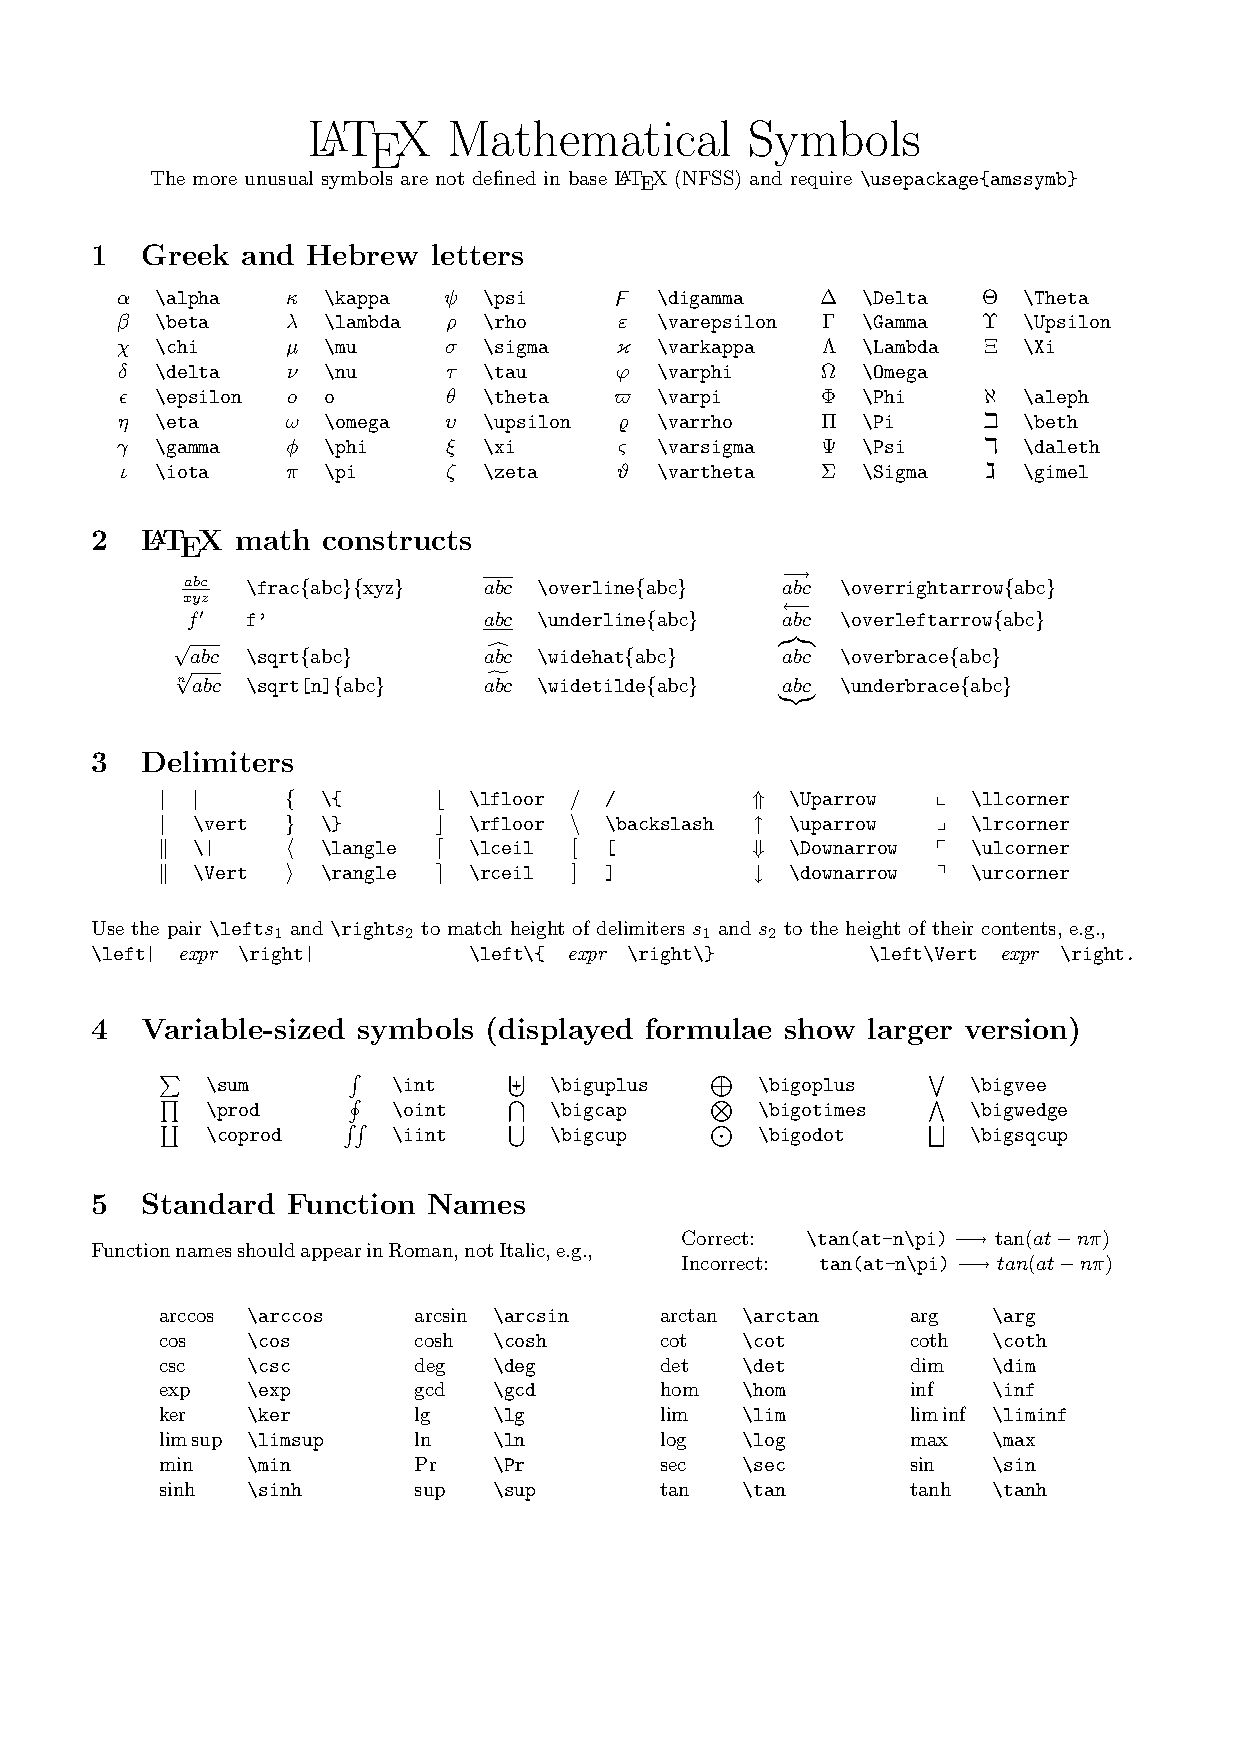
\includepdf[pages=1, pagecommand={\thispagestyle{plain}\subsection{\LaTeX\ Commands} \label{sec:appendixLaTeXSymbols} This section covers common \LaTeX\ commands, reproducing a document created by \citeauthor{LaTeXSymbols} \cite{LaTeXSymbols}.}, width=\linewidth]{Resources/LaTeX-Symbols.pdf}
\includepdf[pages=2-4, pagecommand={\thispagestyle{plain}}, width=\linewidth]{Resources/LaTeX-Symbols.pdf}

\end{document}
